\begin{figure}
	\centering
	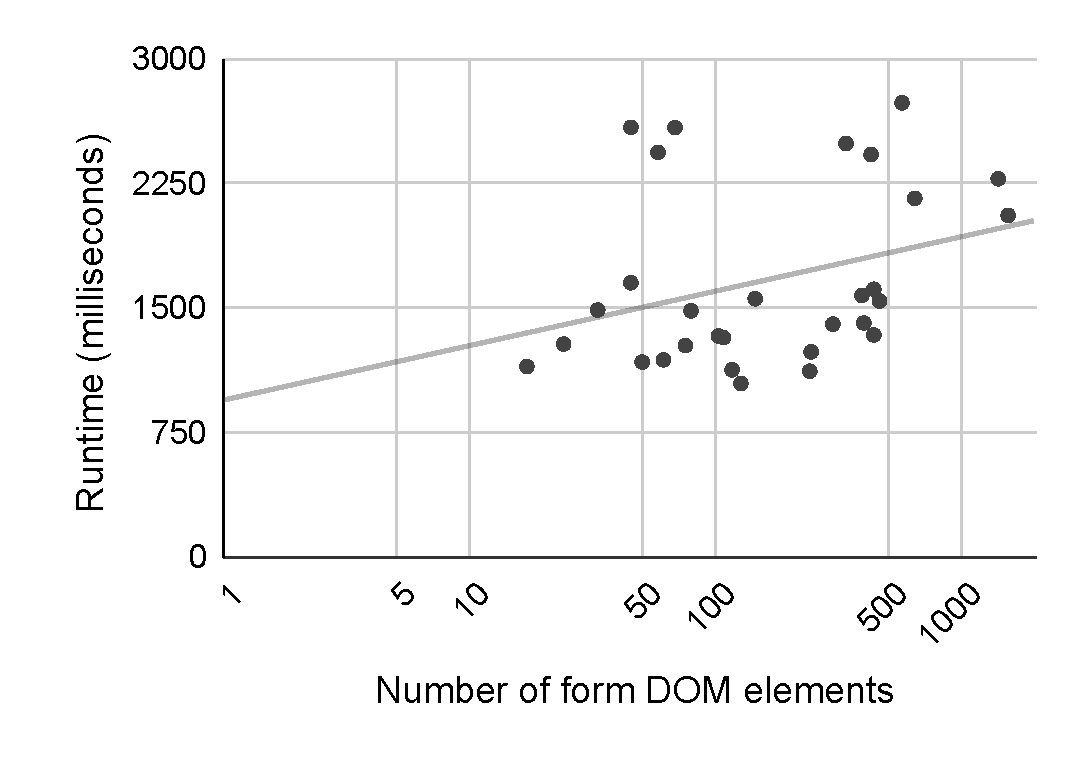
\includegraphics[width=0.7\linewidth,trim={8mm 12mm 8mm 8mm},clip]{accessibility_repair/figures/rq3chart.pdf}
	\caption{Evaluation of the runtime performance scalability for various sizes 
		of input web forms. (Runtime in milliseconds. Form size in number of DOM elements in a form.)}
	\label{fig:rq3}
\end{figure}

\section{Related Work}
A number of tools exist for repairing or improving a few accessibility 
issues~\cite{yesilada2019web, asakawa2019transcoding}. 
One common accessibility improvement approach is already 
in use in modern web browsers, 
such as allowing users with low-vision (e.g., mild vision problems, 
color blindness) to override the default CSS stylesheet into more 
contrasting colors in order to improve their visual perception of 
the page, or to zoom in to the page in order to be able to better 
see its content. Another line of work aims at suggesting alternative 
texts for images to make them accessible~\cite{mack2021designing, 
wu2017automatic, bigham2006webinsight}, building on the abundant 
and extensive deep learning research on the task of image 
captioning~\cite{hossain2019comprehensive}. Accessibility improvements 
have also been proposed based on restructuring of web page regions with 
the goal of prioritizing key sections so that they become more prominent 
and easier to access~\cite{akpinar2015old}.

However, there is little to no work in the literature in terms of a 
software analysis approach that infers and repairs missing web form 
DOM labeling markup, which is one of the most common web accessibility 
errors~\cite{webaim:1mil}. This is the research problem that the presented approach addresses. 

Another line of work focuses on accessibility testing~\cite{abascal2019tools, 
ukgov:audit:2018}, which is generally based on performing syntactic checks 
that consist of basic rules, such as:  any \code{ul} list element must contain 
non-empty \code{li} child elements, or no \code{input} elements must not be 
descendent of \code{a} elements. The goal of such checks is to provide quick 
and simple assertions that are easily automatable.
Patil et al.~\cite{patil2016enhanced} and Eler et al.~\cite{eler2018automated} 
check for absence of predefined attributes in mobile applications, 
such as the absence of required alternative text for all user interface images. 
These are then flagged and reported to developers, allowing them to identify 
and fix these potential issues. Other tools~\cite{aslint_tool,goog_scanner} 
perform similar syntax checks, differing mainly in what attributes are being checked. 
None of these works, however, perform repairs. 

The majority of existing software accessibility related research  
come from a human factors research perspective, rather than from a 
software engineering or tooling perspective.
For instance, one line of work~\cite{snider2020accessibility, alshayban2020accessibility, 
yan2019current, bhagat2019evaluation,ross2018examining,agrawal2019evaluating,dominguez2018website} 
is based on analyzing existing websites (or categories of websites, 
such as educational or banking) by manually 
observing how non-sighted users would interact with them. 
The goal is to discover any issues that might surface during usage, 
and then come up with improved accessibility guidelines. 
The hope is that these guidelines will be later kept in mind while 
developing software. 
A related area of research aims to discover how the software development 
practices themselves can be improved such that it is more likely that 
the end product software is more accessible. 
Krainz et al.~\cite{krainz2018can} explores how model-based development 
contributes to accessibility compliance. 
Sanchez et al.~\cite{sanchez2017method} and Bai et al.~\cite{bai2018categorization, 
bai2019methods} focus on agile software engineering practices and how do they 
impact the accessibility of the product.  

Another line of research is concerned with generating inputs for 
testing purposes~\cite{adamo2018combinatorial,su2017guided}. 
These works have proposed techniques geared towards improving 
the generation, utility, or robustness of test inputs. 
One goal of this vast area of research is to create better 
sequences of test operations or test data with the goal of 
achieving a certain testing objective (e.g., increased coverage). 
\cite{song2017ehb, sadeghi2017pat} adopt a strategy 
of randomly generating the inputs. 
In these cases, the focus is not mainly on the generated input 
data itself but on other aspects of testing, such as improving 
how the event space is traversed or how to better generate 
assertions, with the raw input data being randomly generated, 
or predefined by the user. Another line of work~\cite{arnatovich2018mobolic, 
dhok2016type} gives more attention to the raw input data. 
In these cases, specific types or formats of input values 
are used instead of randomly generated inputs. 
The intuition is that properly formatted and typed inputs 
allow better exploration and testing. 
The aforementioned works, however, are not related to accessibility 
testing or repair, nor aim at generating the required labeling 
associations to be able to perform accessibility repair.  

Finally, a few existing works have explored the use of some visual analysis 
aspects for testing or analyzing web applications. 
Burg et al.~\cite{burg2015explaining} propose a program understanding tool 
that is geared towards front-end development projects and understanding how 
the user interface changes during interactions with the application. It allows 
a developer to select a certain element that 
they are interested in, and the tool tracks how the UI is changing with respect to 
that element, and tracks the corresponding code changes. 
Bajammal et al.~\cite{bajammal2018generating} analyzes the UI of a web page in 
order to generate reusable components, based on patterns in design mockups or templates.  
Choudhary et al.~\cite{choudhary2012crosscheck} focuses on cross-browser 
compatibility, and proposes a technique that checks for difference between 
how a given web page is rendered across browsers. A given web app is loaded in two 
different browsers, and an image diff is performed to locate the areas where 
the two browsers differ, therefore helping the developer to identify issues 
that may not otherwise be easy to identify. 

